\documentclass[border=10pt]{standalone}
\usepackage[svgnames]{xcolor}
\usepackage{amsmath}
\usepackage{pgfplots}
\pgfplotsset{compat=newest}
\usepackage[sfdefault]{FiraSans}
\usepackage{FiraMono}
\renewcommand*\familydefault{\sfdefault}
\begin{document}
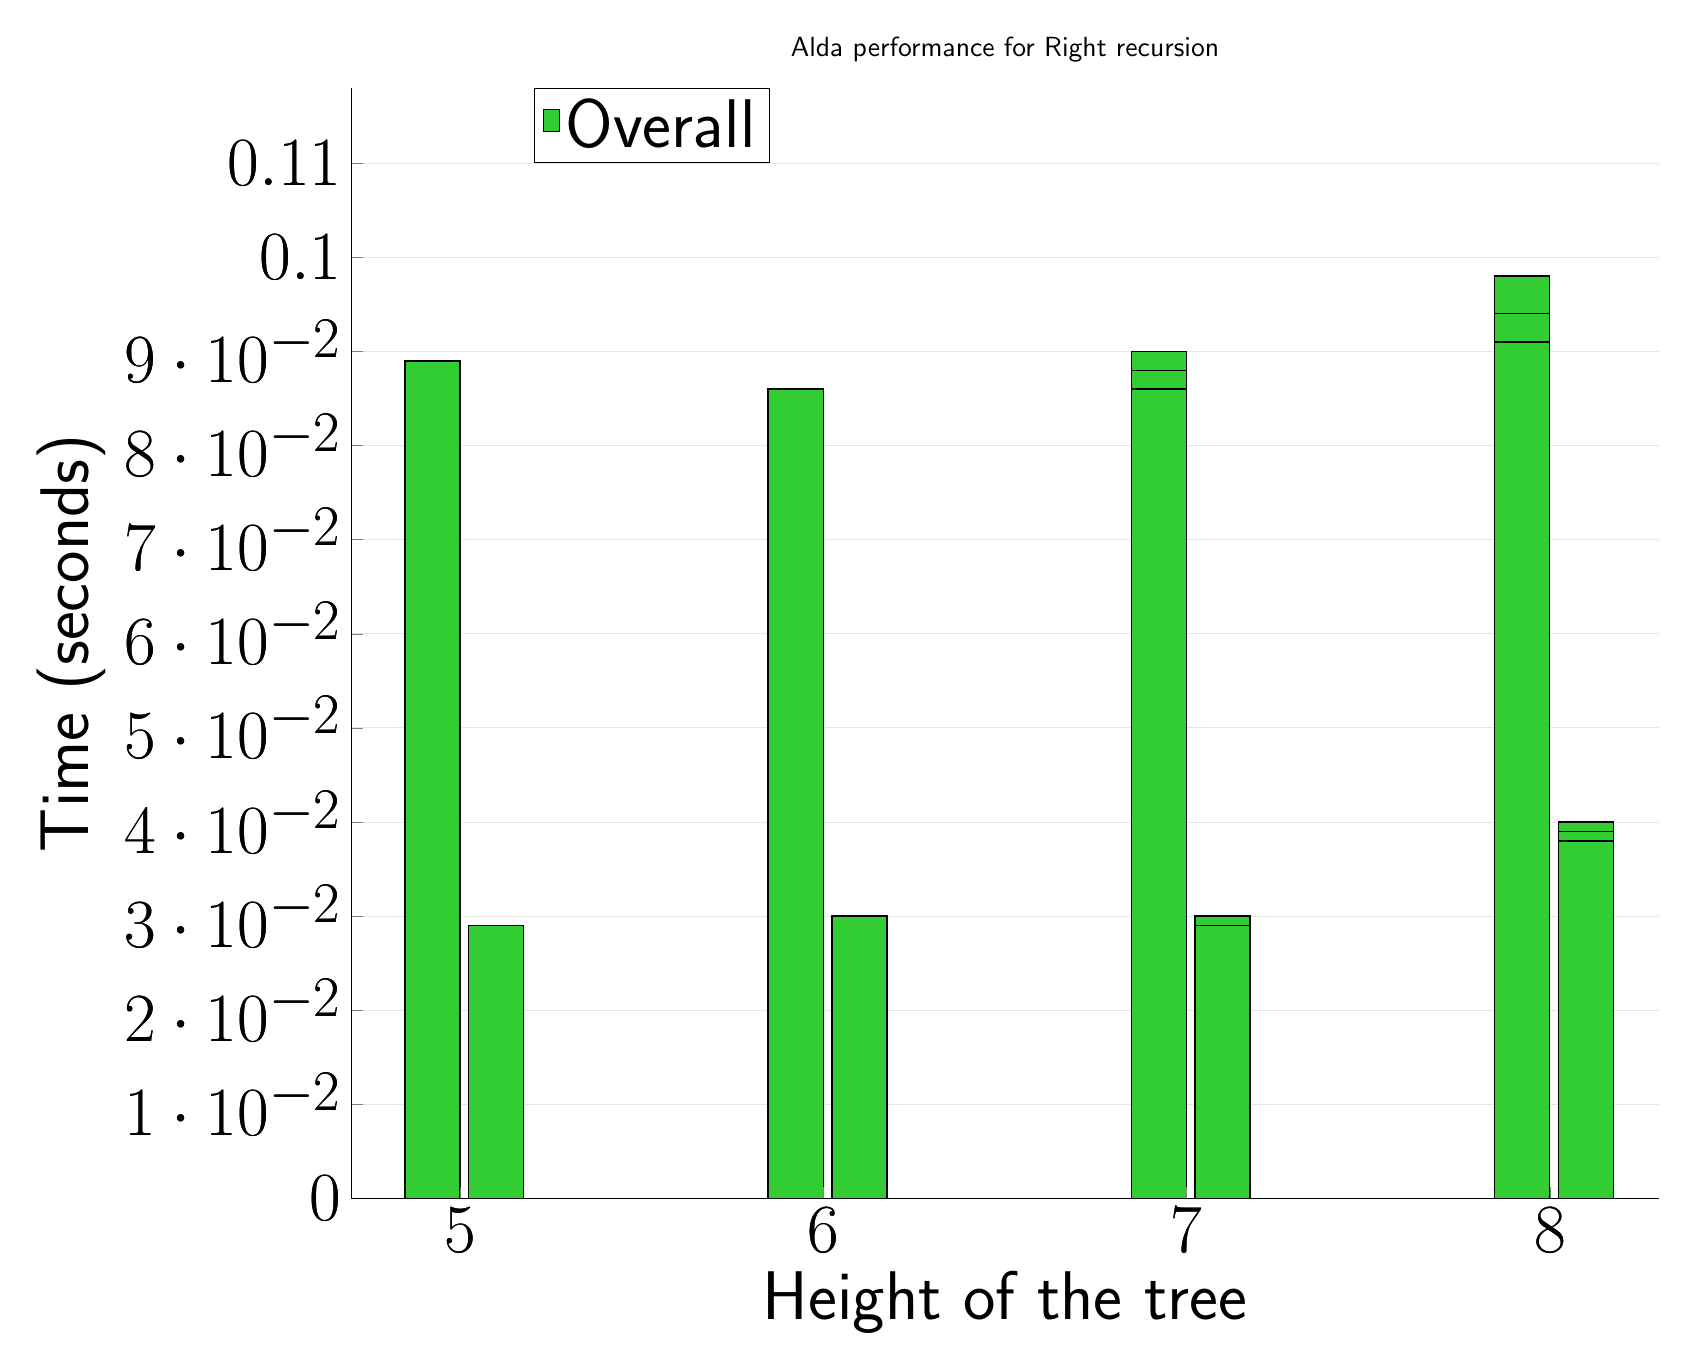
\begin{tikzpicture}
	\begin{axis}[
			ybar stacked,
			title={Alda performance for Right recursion},
			bar shift=-10pt,
			width=1.5\textwidth,
			bar width=0.7cm,
			ymajorgrids, tick align=inside,
			major grid style={draw=gray!20},
			xtick=data,
			ymin=0, ymax=0.11800002574920655,
			axis x line*=bottom,
			axis y line*=left,
			enlarge x limits=0.1,
			legend style={
					at={(0.23, 1)},
					anchor=north,
					legend columns=1,
					font=\Huge,
				},
			ylabel={Time (seconds)},
			xlabel={Height of the tree},
			label style={font=\Huge},
			tick label style={font=\Huge},
		]
		\addlegendimage{fill=LimeGreen, draw=black, line width=0.2pt}
		\addlegendentry{Overall}
		\addplot +[fill=LimeGreen, draw=black, line width=0.5pt] coordinates {
				(5, 0.08899996280670167)
				(6, 0.08599998950958251)
				(7, 0.09000000953674317)
				(7, 0.08799998760223389)
				(7, 0.08599996566772461)
				(8, 0.09099998474121093)
				(8, 0.09800004959106445)
				(8, 0.09399998188018799)
			};
	\end{axis}
	\begin{axis}[
			ybar stacked,
			bar shift=13pt,
			width=1.5\textwidth,
			bar width=0.7cm,
			ymajorgrids, tick align=inside,
			major grid style={draw=none},
			xtick=data,
			ymin=0, ymax=0.11800002574920655,
			axis x line*=none,
			axis y line*=none,
			enlarge x limits=0.1,
			label style={font=\Huge},
			tick label style={font=\Huge},
		]
		\addplot +[fill=LimeGreen, draw=black, line width=0.5pt] coordinates {
				(5, 0.029000000000000005)
				(6, 0.030000000000000006)
				(7, 0.029000000000000005)
				(7, 0.029000000000000005)
				(7, 0.030000000000000006)
				(8, 0.040000000000000015)
				(8, 0.03800000000000001)
				(8, 0.039000000000000014)
			};
	\end{axis}
\end{tikzpicture}

\end{document}
